\documentclass{article}
\usepackage{../../typesetting/styles/report-zh}

% Set document information
\title{周报 向嘉豪 (\today)}
\author{向嘉豪}
\date{\today}

\begin{document}

\maketitle

\begin{abstract}
  本
\end{abstract}

\begin{weekplan}
1)
\end{weekplan}

\section{工作进展}


\section{论文写作}

\subsection{口语表达修正}

在论文撰写过程中,对文本进行了系统性语言风格调整,以提升学术质量和技术准确性。这些修订主要包括:采用更精确的动词表达;删除冗余短语,构建更紧凑的句子结构;改进段落组织,确保每段具有明确的主题句和支持论点;统一使用被动语态以维持学术客观性;优化图表说明,使解释更加直接明了。图\ref{fig:example}展示了这类修订的实例,其中将口语化表达如``is"和``main"分别替换为更专业的术语``represents"和``fundamental",从而增强了文本的学术严谨性。

\begin{figure}[htbp]
\centering
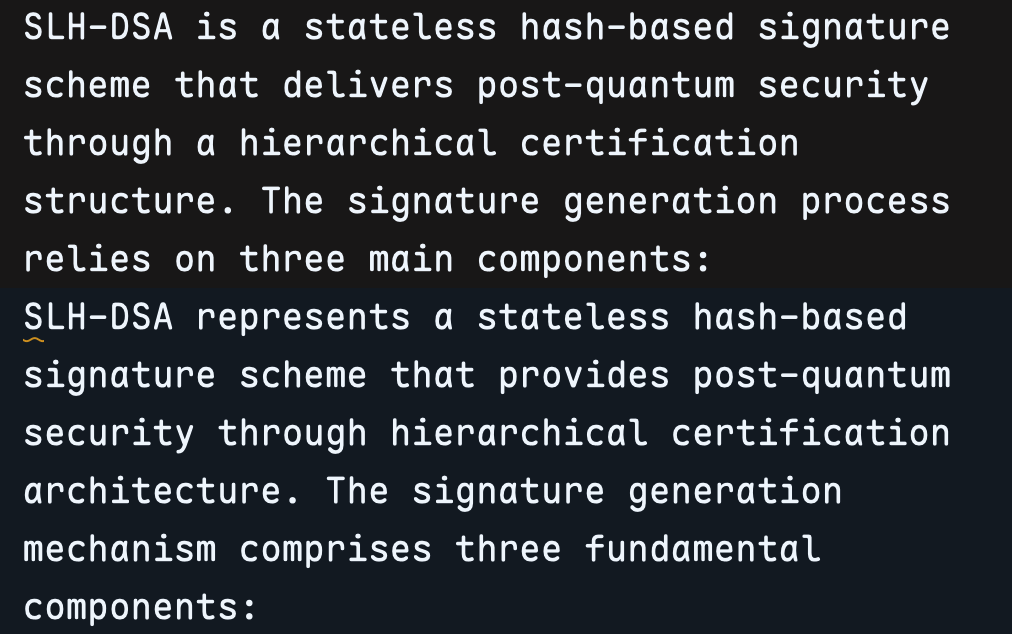
\includegraphics[width=0.5\textwidth]{./fig/fix_writing.png}
\caption{学术语言风格优化示例}
\label{fig:example}
\end{figure}

% Replace standard bibliography commands with conditional version
\printbibliographyifcited[alpha]{../../paper}

\end{document}
